\documentclass{article}

\usepackage{amsmath,amsthm,amssymb} %Misc math symbols
\usepackage{mathtools}
\usepackage[utf8]{inputenc}
\usepackage[margin=1in]{geometry}
\usepackage{caption} 				%Inserting multiple figures
\usepackage{subcaption}
\usepackage[svgnames]{xcolor}
\usepackage{listings}
\usepackage{tikz, pgfplots} 			%Drawing pictures
\usepackage{fancyhdr} 				%Header style
\usepackage[svgnames]{xcolor}		%Coding styles
\usepackage{enumitem}				%Enumerating using letters
\usepackage{mathrsfs}				%Fonts
\usepackage{listings}

\usepackage{accents}
\newcommand{\dbtilde}[1]{\accentset{\approx}{#1}}
\newcommand{\vardbtilde}[1]{\tilde{\raisebox{0pt}[0.85\height]{$\tilde{#1}$}}}

\setlength{\headheight}{15.2pt}
\pagestyle{fancy}
\lhead{ \fancyplain{}{Andrew Kao} }
\rhead{ \fancyplain{}{Autumn 2019} }
\chead{ \fancyplain{}{BUS 41100}}

\begin{document}

\subsection*{Research Question}

The media we consume is critical to shaping our sense of identity, and prior work has highlighted its importance across domains and in multiple contexts: Oberholzer-Gee, Waldfogel (AER 2009) demonstrate that the presence of Spanish language local news increases Hispanic voter turnout, while Yanigazawa-Drott (QJE 2014) shows that radio broadcasts in Rwanda contributed to the violence and genocide that took place in the 90s.

In the next few pages, I aim to examine the causal effect of Spanish language television (SLTV) on schooling outcomes for Hispanic people. Specifically, I look at the potentially adverse discipline consequences that may arise from the presence of television, ranging from out-of-school suspensions to race/ethnicity-based harassment. 


\subsection*{Method and Model}

To isolate the causal effect of Spanish language television, I adopt the technique used in Newman, Velez (AJPS 2019) and generalize it from three counties to the entirety of the US. Newman and Velez exploit a FCC (Federal Communications Commission) regulation which determines the distance from a TV station in which the station's broadcast signal is protected from interference. This creates a natural regression discontinuity, where the decaying strength of a signal over distance is combined with this cutoff in broadcast protection to create a split among people just inside and outside these coverage 'contours' that are presumably comparable save for their access to broadcast TV. 


\begin{figure}[!hbtp]
\centering
\caption{The Coverage Contours of Spanish Language TV stations}
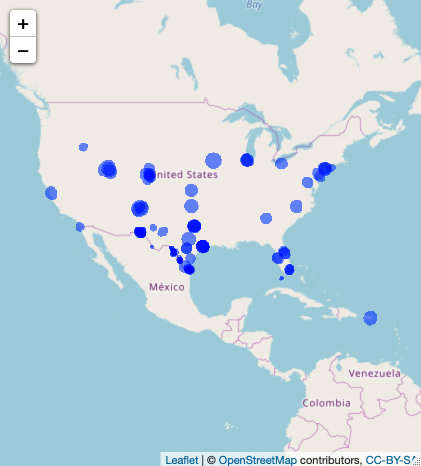
\includegraphics[width=8cm]{../analysis/Output/img/SpanishContours.png}
\end{figure} 

In the case of Spanish language TV in particular, this should allow me to examine its causal effect on Hispanic populations for spatially located outcomes, such as public schooling results. It's worth noting that these contours are purely determined by an algorithm that looks at things like local elevation and antennae strength, so that the cutoffs are located in more or less random locations, and that coverage is large enough that these contours tend to cut across towns and suburbs, rather than cities. % Finally, regressions using US census data indicate that Hispanic people do not migrate across counties in response to these contours.

A standard regression thus looks like restricting the universe of schools to only those within a small radius of the contour boundary, where the key independent variable of interest is an indicator for the school being inside or outside the boundary, interacted with the distance to the boundary:
\[ Y_i^{j,k} = \beta_0 + \beta \mathbb{I}[InsideContour_i] \times Distance_i + \gamma X_i + \delta Z^j + \epsilon_i^k \, \, \, \, \, \, \, \epsilon \stackrel{iid}{\sim}   N(0,\sigma_i^{k^2})\]

where $Y_i$ is an outcome for school $i$ in county $j$ and school district $k$, $X$ is a vector of school-level controls, and $Z$ is a vector of county-level controls. Errors are often clustered by school district, meaning that $Corr(\sigma_i^k, \sigma_{i'}^k) \neq 0$ is permissible.

When the outcome variable is a binary variable, the model instead follows:
\[\mathbb{P}(Y_i^j = 1 | X,Z) = \frac{\exp[\beta_0 + \beta \mathbb{I}[InsideContour_i] \times Distance_i + \gamma X_i + \delta Z^j ] }{ 1 + \exp[\beta_0 + \beta \mathbb{I}[InsideContour_i] \times Distance_i + \gamma X_i + \delta Z^j ]}\]

for a logistic/logit regression. 

\subsection*{Data}

Data for the instrument comes from both the FCC and TMS (a telecommunications company that was kind enough to let me use their API for free). The relevant data here is essentially just the coverage contour spatial data and the broadcast language of the station.


The data on public schools comes from the US government's CRDC (Civil Rights Data Collection) dataset. It's a very large dataset with over 500 outcome/control variables (the vast majority of these are not suitable as controls for one another in this setting), and importantly, it breaks down all major variables of interest by ethnicity. These are all at the school level, and the geographic location of these schools is mapped using ArcGIS. 

\begin{figure}[!hbtp]
\centering
\caption{Map of School Districts in the US}
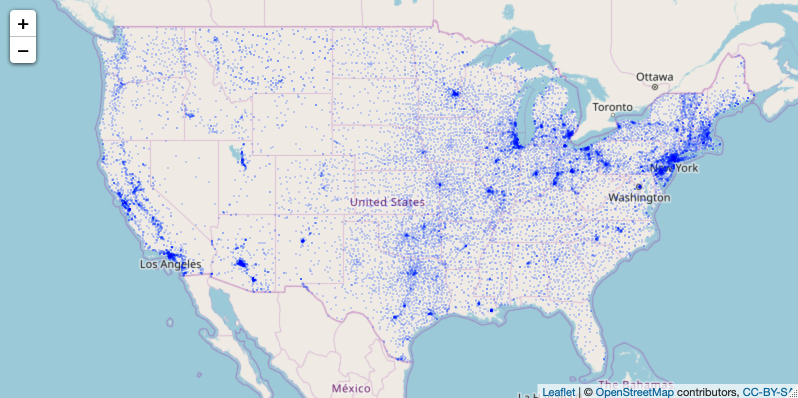
\includegraphics[width=12cm]{../analysis/Output/img/LEAMap.png}
\end{figure} 

Additional controls like population, income, density of Hispanic population etc. at the county level are from IPUMS.

Some summary statistics of interest are presented below:

\clearpage

% Table created by stargazer v.5.2.2 by Marek Hlavac, Harvard University. E-mail: hlavac at fas.harvard.edu
% Date and time: Fri, Dec 13, 2019 - 20:45:59
\begin{table}[!htbp] \centering 
  \caption{School-District Level Summary Statistics} 
  \label{} 
\begin{tabular}{@{\extracolsep{5pt}}lccccccc} 
\\[-1.8ex]\hline 
\hline \\[-1.8ex] 
Statistic & \multicolumn{1}{c}{N} & \multicolumn{1}{c}{Mean} & \multicolumn{1}{c}{St. Dev.} & \multicolumn{1}{c}{Min} & \multicolumn{1}{c}{Pctl(25)} & \multicolumn{1}{c}{Pctl(75)} & \multicolumn{1}{c}{Max} \\ 
\hline \\[-1.8ex] 
Distance to Boundary & 17,280 & 136.855 & 146.751 & 0.000 & 15.786 & 217.567 & 806.543 \\ 
SLTV Coverage Dummy & 17,280 & 0.292 & 0.455 & 0.000 & 0.000 & 1.000 & 1.000 \\ 
\% County Hispanic & 17,280 & 7.051 & 11.950 & 0.000 & 0.668 & 6.974 & 97.216 \\ 
Log(Population) & 17,280 & 11.618 & 1.840 & 5.869 & 10.242 & 13.110 & 15.997 \\ 
Log(Income) & 17,280 & 9.428 & 0.257 & 7.976 & 9.257 & 9.593 & 10.245 \\ 
\hline \\[-1.8ex] 
\multicolumn{8}{l}{\textit{Note:} Distance to SLTV Boundary measured in KM} \\ 
\end{tabular} 
\end{table} 


% Table created by stargazer v.5.2.2 by Marek Hlavac, Harvard University. E-mail: hlavac at fas.harvard.edu
% Date and time: Fri, Dec 13, 2019 - 22:32:28
\begin{table}[!htbp] \centering 
  \caption{School Level Summary Statistics} 
  \label{} 
\begin{tabular}{@{\extracolsep{5pt}}lccccccc} 
\\[-1.8ex]\hline 
\hline \\[-1.8ex] 
Statistic & \multicolumn{1}{c}{N} & \multicolumn{1}{c}{Mean} & \multicolumn{1}{c}{St. Dev.} & \multicolumn{1}{c}{Min} & \multicolumn{1}{c}{Pctl(25)} & \multicolumn{1}{c}{Pctl(75)} & \multicolumn{1}{c}{Max} \\ 
\hline \\[-1.8ex] 
Total Students & 96,349 & 524.859 & 449.354 & 2.000 & 254.000 & 662.000 & 14,164.000 \\ 
\# Hispanic Students & 91,019 & 143.195 & 243.873 & 2.000 & 13.000 & 166.000 & 7,675.000 \\ 
Contains Grade 1 & 96,350 & 0.538 & 0.499 & 0 & 0 & 1 & 1 \\ 
Contains Grade 6 & 96,350 & 0.364 & 0.481 & 0 & 0 & 1 & 1 \\ 
Contains Grade 9 & 96,350 & 0.253 & 0.435 & 0 & 0 & 1 & 1 \\ 
Hispanic Suspension Dummy & 94,535 & 0.382 & 0.486 & 0.000 & 0.000 & 1.000 & 1.000 \\ 
Hispanic Chronic Absentees & 94,540 & 22.920 & 57.838 & 0.000 & 0.000 & 22.000 & 2,131.000 \\ 
\# Teachers & 93,934 & 35.219 & 33.892 & 1.000 & 19.000 & 44.000 & 6,031.000 \\ 
\hline \\[-1.8ex] 
\multicolumn{8}{l}{\textit{Note:} Dummies indicate whether event occurred in the school over the past year} \\ 
\end{tabular} 
\end{table} 

\clearpage

\subsection*{}



%
% Table created by stargazer v.5.2.2 by Marek Hlavac, Harvard University. E-mail: hlavac at fas.harvard.edu
% Date and time: Wed, Nov 13, 2019 - 15:16:32
\begin{table}[!htbp] \centering 
  \caption{GED Completions} 
  \label{} 
\begin{tabular}{@{\extracolsep{5pt}}lccccccc} 
\\[-1.8ex]\hline 
\hline \\[-1.8ex] 
Statistic & \multicolumn{1}{c}{N} & \multicolumn{1}{c}{Mean} & \multicolumn{1}{c}{St. Dev.} & \multicolumn{1}{c}{Min} & \multicolumn{1}{c}{Pctl(25)} & \multicolumn{1}{c}{Pctl(75)} & \multicolumn{1}{c}{Max} \\ 
\hline \\[-1.8ex] 
LEA\_GEDPART\_HI\_M & 656 & 12.901 & 77.293 & 0 & 0 & 5 & 1,550 \\ 
LEA\_GEDPART\_HI\_F & 656 & 10.869 & 66.649 & 0 & 0 & 5 & 1,136 \\ 
TOT\_GEDPART\_M & 656 & 53.639 & 173.840 & 2 & 10 & 51.2 & 3,485 \\ 
TOT\_GEDPART\_F & 656 & 39.765 & 136.175 & 0 & 5 & 37 & 2,225 \\ 
LEA\_GEDCRED\_HI\_M & 656 & 2.130 & 18.292 & $-$2 & $-$2 & $-$2 & 298 \\ 
LEA\_GEDCRED\_HI\_F & 656 & 1.201 & 16.312 & $-$2 & $-$2 & $-$2 & 253 \\ 
TOT\_GEDCRED\_M & 656 & 20.870 & 55.866 & 4 & 4 & 17 & 793 \\ 
TOT\_GEDCRED\_F & 656 & 13.791 & 43.218 & $-$2 & $-$2 & 11 & 619 \\ 
\hline \\[-1.8ex] 
\end{tabular} 
\end{table} 


%
% Table created by stargazer v.5.2.2 by Marek Hlavac, Harvard University. E-mail: hlavac at fas.harvard.edu
% Date and time: Wed, Nov 13, 2019 - 15:16:32
\begin{table}[!htbp] \centering 
  \caption{GED Completions} 
  \label{} 
\begin{tabular}{@{\extracolsep{5pt}}lccccccc} 
\\[-1.8ex]\hline 
\hline \\[-1.8ex] 
Statistic & \multicolumn{1}{c}{N} & \multicolumn{1}{c}{Mean} & \multicolumn{1}{c}{St. Dev.} & \multicolumn{1}{c}{Min} & \multicolumn{1}{c}{Pctl(25)} & \multicolumn{1}{c}{Pctl(75)} & \multicolumn{1}{c}{Max} \\ 
\hline \\[-1.8ex] 
LEA\_GEDPART\_HI\_M & 656 & 12.901 & 77.293 & 0 & 0 & 5 & 1,550 \\ 
LEA\_GEDPART\_HI\_F & 656 & 10.869 & 66.649 & 0 & 0 & 5 & 1,136 \\ 
TOT\_GEDPART\_M & 656 & 53.639 & 173.840 & 2 & 10 & 51.2 & 3,485 \\ 
TOT\_GEDPART\_F & 656 & 39.765 & 136.175 & 0 & 5 & 37 & 2,225 \\ 
LEA\_GEDCRED\_HI\_M & 656 & 2.130 & 18.292 & $-$2 & $-$2 & $-$2 & 298 \\ 
LEA\_GEDCRED\_HI\_F & 656 & 1.201 & 16.312 & $-$2 & $-$2 & $-$2 & 253 \\ 
TOT\_GEDCRED\_M & 656 & 20.870 & 55.866 & 4 & 4 & 17 & 793 \\ 
TOT\_GEDCRED\_F & 656 & 13.791 & 43.218 & $-$2 & $-$2 & 11 & 619 \\ 
\hline \\[-1.8ex] 
\end{tabular} 
\end{table} 





\end{document}
























